\section{Approach}
\label{sec:Approach}

As previously mentioned, a module that implements an LST scheduler is
optimal for multi-core system, even though it is practically
infeasible to be implemented at a fine granularity at an OS
level. This is mainly because an active accounting for the slack time
of each job in the system need to be performed (see
Section~\ref{sec:Objective}).

In this work, we propose to use an hybrid platform to benefit from a
multi-core embedded processor while at the same time being able to
implement a dedicated hardware LST scheduler. Specifically, we are
targeting the ZedBoard development board based on the Xilinx Zynq
Z-7020 SoC which features a dual-core ARM Cortex-A9 MPCore which
operates at a frequency of 667~MHz. The main CPU is coupled with an
Artix 7 FPGA featuring 85k logic cells and including 140 blocks of RAM
of 36~Kb each; 220 DSP slices and 2 12-bit ADCs.

\begin{figure}[h]
  \centering
  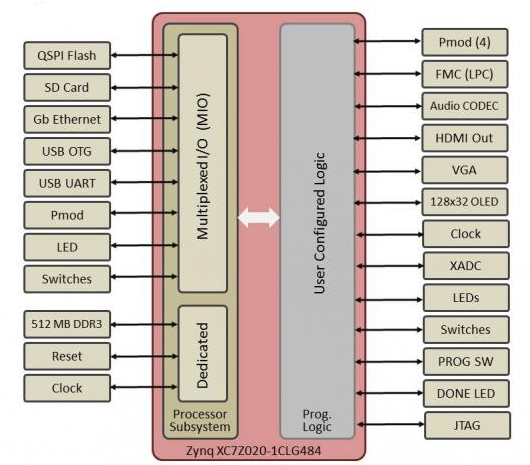
\includegraphics[width=0.4\textwidth]{fig/blocks.png}
  \caption{Block-view of the ZedBoard evaluation platform.}
  \label{fig:blocks}
\end{figure}

The block view of the internal organization of the targeted board is
depicted in Figure~\ref{fig:blocks}. As can be seen, the block of
programmable logic can be used to both change the interconnections of
the processor subsystem with the I/O peripherals and implement custom
user-defined additional logic. Thus, we intend to deploy our LST
scheduler inside the FPGA block and having a fully operating dual-core
embedded processor.

Linux could be selected as the OS that runs on top of the embedded
CPU. This would have the great advantege of enabling a fast
development of user-space benchmarking applications and a full
interactivity with a wide range of I/O peripherals. Unfortunately,
however, the Linux kernel heavily relies on periodic timer interrupts
to perform scheduling, book-keeping of resources and interact with I/O
devices. Since our aim is to explore the benefits of a system design
that do not interrupt the CPU to perform schedulability since it can
rely on a dedicated hardware module, the option of using a Linux OS
present several disadvantages. In particular, it would require a
non-trivial time to modify the Linux kernel so to exclude the
scheduling features while implementing a backward compatible shceduler
in hardware. 

\begin{figure}[h]
  \centering
  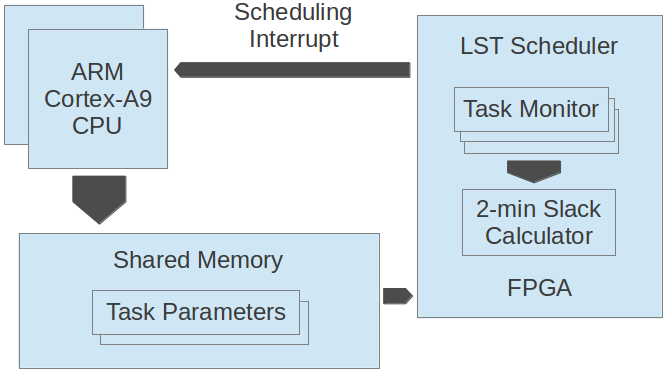
\includegraphics[width=0.4\textwidth]{fig/sched.png}
  \caption{Overview of the proposed architecture..}
  \label{fig:arch}
\end{figure}

For this reason, we follow the approach of using a bare-metal OS which
provides basic primitives for the definition of tasks, interaction
with devices and debugging. Moreover, the bare-metal OS does not
implement any scheduling primitive. In fact, it completely relies on
an interface with the hardware scheduler to schedule/de-schedule
tasks.

An overview of the structure of the overall system is provided in
Figure~\ref{fig:arch}. The bare-metal OS running on the embedded
processor exports at startup the parameter of the tasks on a block of
shared memory. The LST scheduler read the task parameters and
instantiates a number of hardware task monitors accordingly. Next, the
LST scheduler computes the 2 jobs that need to be scheduled by quering
the task monitors an determining which one is the task with the
minimum slack. Whenever the hardware module detect that a different
task from the one that is being currently executed has to be
scheduled, it generates an interrupt for the targeted core. A fast
interrupt handler in the ARM core reads the ID of the new task that
has to be scheduled and performs the context-switch accordingly.
